\documentclass[preprint2]{aastex631}
\received{\today}
\shorttitle{Inside-Out Growth in the Milky Way Disc}
\graphicspath{{figures/}}

\usepackage{lipsum}
\usepackage{physics}
\usepackage{multirow}
\usepackage{xspace}
\usepackage{natbib}
\usepackage{fontawesome5}
\usepackage{xcolor}
\usepackage{wrapfig}
\usepackage[figuresright]{rotating}

% remove indents in footnotes
\usepackage[hang,flushmargin]{footmisc} 

\newcommand{\todo}[1]{{\color{red}{[TODO: #1}]}}
\newcommand{\needcite}{{\color{magenta}{(needs citation)}}}
\newcommand{\placeholder}[1]{{\color{gray} \lipsum[#1]}}

% custom function for adding units
\makeatletter
\newcommand{\unit}[1]{%
    \,\mathrm{#1}\checknextarg}
\newcommand{\checknextarg}{\@ifnextchar\bgroup{\gobblenextarg}{}}
\newcommand{\gobblenextarg}[1]{\,\mathrm{#1}\@ifnextchar\bgroup{\gobblenextarg}{}}
\makeatother

\begin{document}

\title{{\Large Inside-Out Growth in the Milky Way Disc}\\\vspace{0.15cm}ASTR 511 Final Project}

% affiliations
\newcommand{\UW}{Department of Astronomy, University of Washington, Seattle, WA, 98195}

\author[0000-0001-6147-5761]{Tom Wagg}
\affiliation{\UW}

\correspondingauthor{Tom Wagg}
\email{tomwagg@uw.edu}

\section{Introduction}
For my project I'm going to investigate the inside-out growth of galaxies, focussing specifically on the Milky Way. This is the idea that star formation in galaxies occurs first in the centre and builds outwards.

\section{Background/Early Theories}
\citep{Larson+1976}

\section{Observations}
\subsection{For}
\citep{vanDokkum+2013}
\subsection{Against}
\citep{Goddard+2017}

\section{Models}
\citep{Frankel+2019}

\section{Applications}
\citep{Banerjee+2020}

\section{Future Work}
\citep{Hogg+2019}

% \begin{figure}[htb]
%     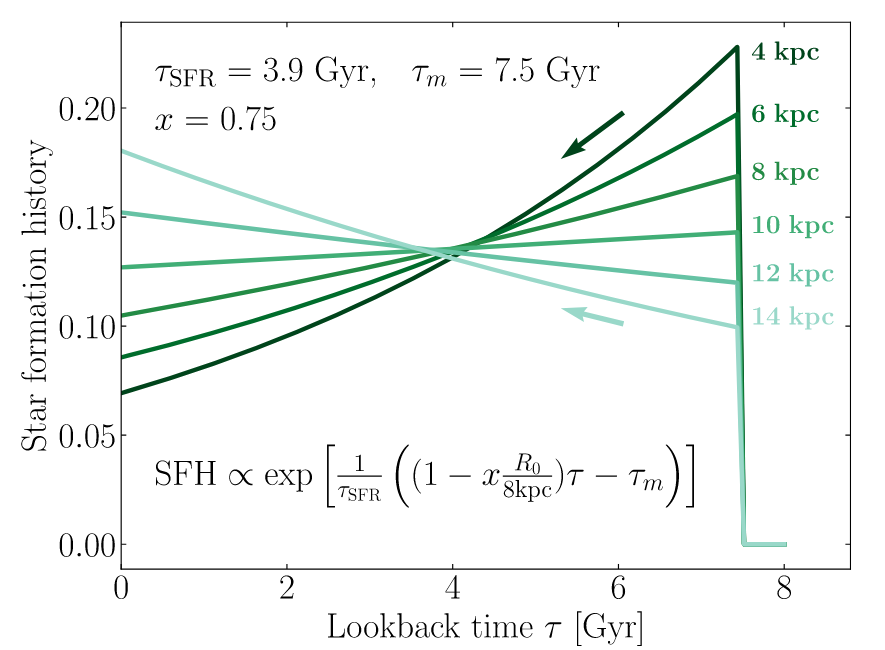
\includegraphics[width=\columnwidth]{frankel2019_fig5.png}
%     \caption{\citet{Frankel+2019} Figure 5 showing the model for inside-out growth.}
% \end{figure}

\bibliographystyle{aasjournal}
\bibliography{refs}{}

\end{document}